\chapter{Opstilling}
\label{cha:opstilling}

En stråle af protoner accelereres op til den ønskede energi med en 5\MV Van de Graaf
accelerator. Denne stråle afbøjes med en eletromagnet og sendes ind i \beamline, hvor det først
passerer gennem et hul i midten af den ene detektor. En del af strålen vil kollidere med et
\SI[per-mode = symbol]{20}{\micro\gram\per\cm\squared} \ce{^{11}B}-\target placeret på
\SI[per-mode = symbol]{4}{\micro\gram\per\cm\squared} kulstof bagbeklædning.  Det resterende vil
passere videre gennem \beamline, hvor det igen vil passere gennem en detektor, for at ende i et
Faradaybæger. Opstillingen er skitseret på \cref{fig:opstilling}.
\begin{figure}[h]
  \centering
  \fxfatal{Detektorerne skal lige tegnes på det rette sted.}
  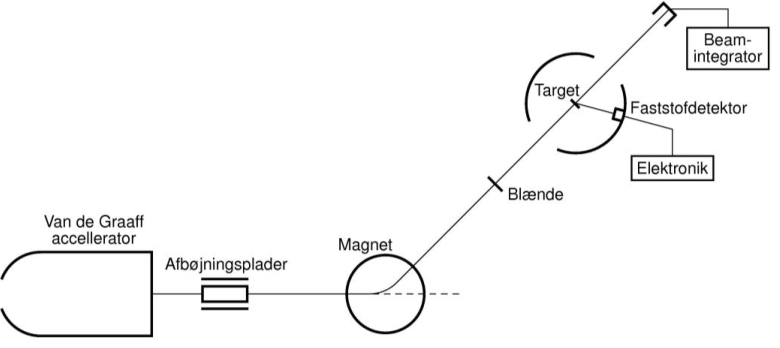
\includegraphics[width=0.7\columnwidth]{Opstilling}
  \caption{Skematisk tegning af opstillingen. Figuren er lånt fra \cite{Knudsen}.}
  \label{fig:opstilling}
\end{figure}

Detektorsystemet består af to dobbeltsidet silicium strip detektorer (DSSSD) af typen S3 fra Micron
Semiconductors Limited \cite{micron-s3}.    Disse
fungerer på samme måde som almindelige fastofdetektorer, og en skematisk tegning af detektoren ses
på \cref{fig:S3}.  Fordelen ved disse detektorer er opdelingen af forsiden og bagsiden i et antal
områder kaldet strips. Dermed er det muligt at optage et positionsfølsomt spektrum af
partiklerne. Bagsiden er opdelt i 32 radiale sektorer. Forsiden er derimod
opdelt i en række ringe, der hver er 886\um tykke, adskilt af et 100\um isolerende område.
\begin{figure}[hbt]
  \centering
  \fxfatal{Her mangler en tegning af W1-detektoren}
  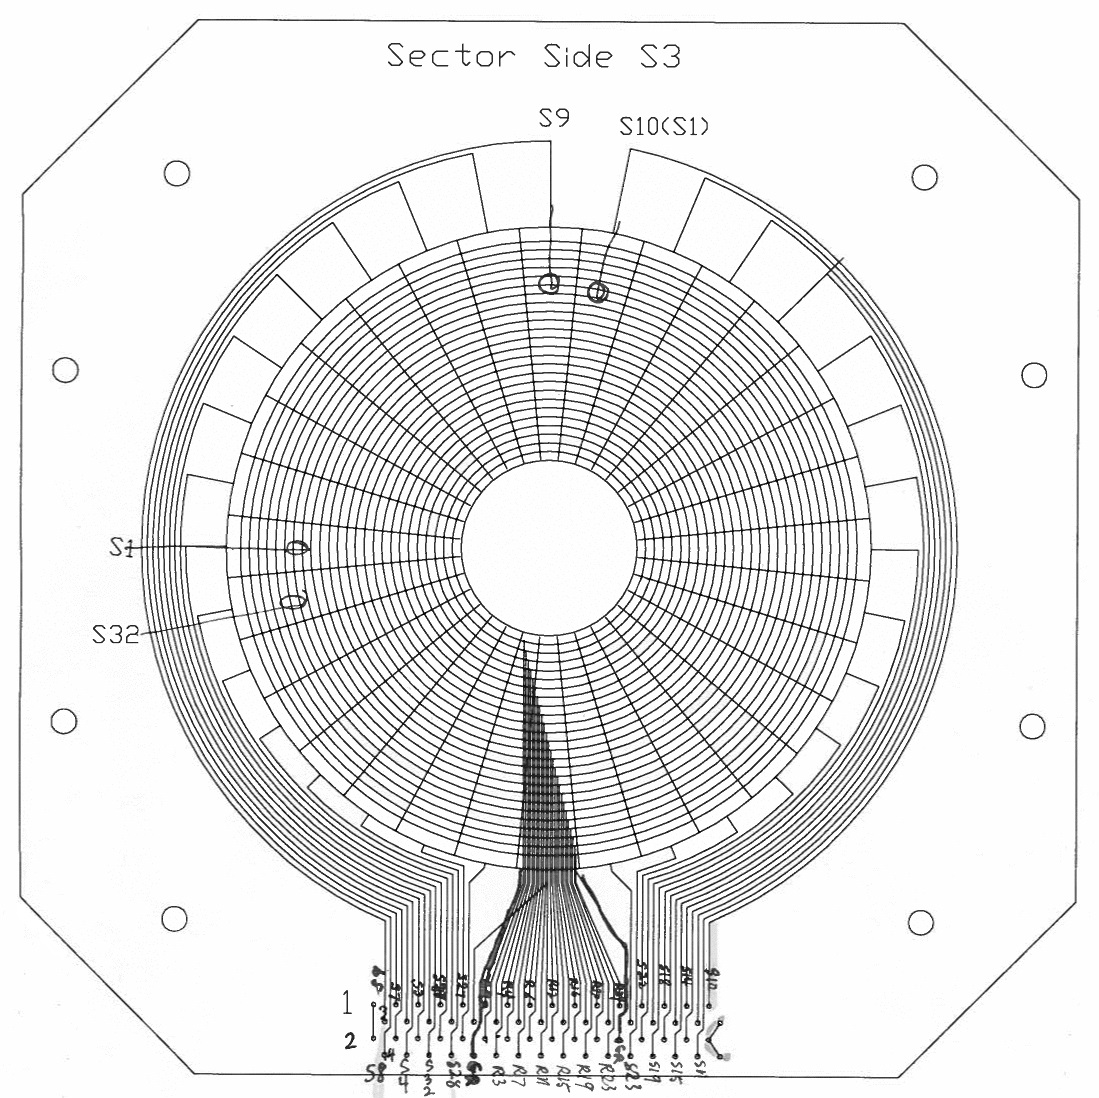
\includegraphics[width=0.5\columnwidth]{S3}
  \caption{Skematisk tegning af S3 detektoren, hvor de 24 ringe og 32 sektorer ses. Bemærk at
  ringene og sektorerne er placeret på hhv. forsiden og bagsiden af detektoren.}
  \label{fig:S3}
\end{figure}

Den første detektor strålen passerer igennem vil blive omtalt som opstrøms, og den udspænder
polarvinklerne, målt ifht. \beamline, fra $141\degree$ til $165\degree$. Den anden detektor benævnes
med nedstrøms og den udspænder fra $15\degree$ til $40\degree$.

\fxfatal{Indfør detektornummerering!}
På begge sidder var der endvidere placeret to W1 DSSSD detektorer også fra Micron \cite{micron-W1}. Disse dektorer er
firkantede og det aktive område måler ${\SI{49.5}{\mm} \times \SI{49.5}{\mm}}$. De to sider er
opdelt i 16 strips af \SI{3000.0}{\um} adskilt af et \SI{0.1}{\mm} isolerende område. Stripsne på
forsiden og bagsiden er placeret vinkelret i forhold til hinanden, hvormed disse dektorer også er
positionsfølsomme i to dimensioner. Med en pixelstørrelse \SI{9}{\mm\squared} 

Detektorerne er forbundet til en forforstærker, der er placeret tæt ved for at undgå støj. Signallet
fra disse er ført videre til en analog til digital konverter (ADK) som til sidst er ført til
computeren. Endvidere blev signalerne ført ind i et logisk kredsløb. Udgangssignallet fra denne blev
brugt som triggersignal til ADK'erne. Det logiske kredsløb havde to indstillinger; \lAND og \lOR. Er
den indstillet på \lAND, så skal der være signal i to forskellige detektorer før der kommer et
udgangssignal, hvor der ved \lOR kun skal være signal i en enkelt. Dette gør det muligt at
grovsortere, således at de fleste Rutherfordspredte protoner ikke medtages i det endelige
datasæt. 